\documentclass[12pt]{article}
\usepackage[margin=1in]{geometry}

% Start of preamble
%==========================================================================================%
% Required to support mathematical unicode
\usepackage[warnunknown, fasterrors, mathletters]{ucs}
\usepackage[utf8x]{inputenc}

\usepackage[dvipsnames,table,xcdraw]{xcolor}
\usepackage{hyperref} 
\hypersetup{
	colorlinks=true,
	linkcolor=blue,
	filecolor=magenta,      
	urlcolor=cyan,
	pdfpagemode=FullScreen
}

% Standard mathematical typesetting packages
\usepackage{amsmath,amssymb,amscd,amsthm,amsxtra, pxfonts}
\usepackage{mathtools,mathrsfs,dsfont,xparse}

% Symbol and utility packages
\usepackage{cancel, textcomp}
\usepackage[mathscr]{euscript}
\usepackage[nointegrals]{wasysym}
\usepackage{apacite}

% Extras
\usepackage{physics}  
\usepackage{tikz-cd} 
\usepackage{microtype}
\usepackage{enumitem}
\usepackage{titling}
\usepackage{graphicx}

% Fancy theorems due to @intuitively on discord
\usepackage{mdframed}
\newmdtheoremenv[
backgroundcolor=NavyBlue!30,
linewidth=2pt,
linecolor=NavyBlue,
topline=false,
bottomline=false,
rightline=false,
innertopmargin=10pt,
innerbottommargin=10pt,
innerrightmargin=10pt,
innerleftmargin=10pt,
skipabove=\baselineskip,
skipbelow=\baselineskip
]{mytheorem}{Theorem}

\newenvironment{theorem}{\begin{mytheorem}}{\end{mytheorem}}

\newtheorem{corollary}{Corollary}
\newtheorem{lemma}{Lemma}

\newtheoremstyle{definitionstyle}
{\topsep}%
{\topsep}%
{}%
{}%
{\bfseries}%
{.}%
{.5em}%
{}%
\theoremstyle{definitionstyle}
\newmdtheoremenv[
backgroundcolor=Violet!30,
linewidth=2pt,
linecolor=Violet,
topline=false,
bottomline=false,
rightline=false,
innertopmargin=10pt,
innerbottommargin=10pt,
innerrightmargin=10pt,
innerleftmargin=10pt,
skipabove=\baselineskip,
skipbelow=\baselineskip,
]{mydef}{Definition}
\newenvironment{definition}{\begin{mydef}}{\end{mydef}}

\newtheorem*{remark}{Remark}

\newtheorem*{example}{Example}

% Common shortcuts
\def\mbb#1{\mathbb{#1}}
\def\mfk#1{\mathfrak{#1}}

\def\bN{\mbb{N}}
\def \C{\mbb{C}}
\def \R{\mbb{R}}
\def\bQ{\mbb{Q}}
\def\bZ{\mbb{Z}}
\def \cph{\varphi}
\renewcommand{\th}{\theta}
\def \ve{\varepsilon}
\newcommand{\mg}[1]{\| #1 \|}

% Often helpful macros
\newcommand{\floor}[1]{\left\lfloor#1\right\rfloor}
\newcommand{\ceil}[1]{\left\lceil#1\right\rceil}
\renewcommand{\qed}{\hfill\qedsymbol}
\renewcommand{\P}{\mathbb P\qty}
\newcommand{\E}{\mathbb{E}\qty}
\newcommand{\Cov}{\mathrm{Cov}\qty}
\newcommand{\Var}{\mathrm{Var}\qty}

% Sets
\usepackage{braket}

\graphicspath{{/}}
\usepackage{float}

% End of preamble
%==========================================================================================%

% Start of commands specific to this file
%==========================================================================================%

%==========================================================================================%
% End of commands specific to this file

\title{CSE 446HW0}
\date{\today}
\author{Rohan Mukherjee}

\begin{document}
	\maketitle
	\begin{enumerate}[leftmargin=\labelsep]
		\item By Bayes rule,
		\begin{align*}
			\P(\text{has disease} \mid \text{positive test}) = \frac{\P(\text{pos} \mid \text{disease}) \cdot \P(\text{disease})}{\P(\text{pos})} = \frac{0.99 \cdot 0.0001}{\P(\text{pos})}
		\end{align*}
		By the law of total probability, we have 
		\begin{align*}
			\P(\text{pos}) &= \P(\text{pos} \mid \text{disease}) \cdot \P(\text{disease}) + \P(\text{pos} \mid \text{doesn't}) \cdot \P(\text{doesn't})
			\\& 0.99 \cdot 0.0001 + (1-0.99) \cdot 0.9999
		\end{align*}
		Since $\P(\text{not pos} \mid \text{doesn't}) = 0.99$ we have $\P(\text{pos} \mid \text{doesn't}) = 1-0.99$. Combining these results yields:
		$\P(\text{has disease} \mid \text{positive test}) = \frac{0.99 \cdot 0.0001}{0.99 \cdot 0.0001 + (1-0.99) \cdot 0.9999} \approx 0.009803 \approx .98\%$.
		
		\item 
		\begin{enumerate}
			\item Notice that
			\begin{align*}
				\Cov(X,Y) &= \E[XY - X\E[Y] - Y\E[X] - \E[X]\E[Y]] 
				\\&= \E[XY] - \E[X]\E[Y] - \E[X]\E[Y] + \E[X]\E[Y] 
				\\&= \E[XY] - \E[X]\E[Y]
			\end{align*}
			First, by the law of total expectation,
			\begin{align*}
				\E[Y] &= \int_\R \E[Y \mid X = x] p_X(x)dx
				\\&= \int_\R x  p_X(x)dx = \E[X]
			\end{align*}
			By the same law,
			\begin{align*}
				\E[XY] &= \int_\R \E[XY \mid X = x]p_X(x)dx
				\\&= \int_\R \E[x \cdot Y \mid X = x] p_X(x)dx 
				\\&= \int_\R x\E[Y \mid X = x] p_X(x)dx \quad \text{By lineararity of expectation} 
				\\&= \int_\R x^2 p_X(x)dx = \E[X^2]
			\end{align*}
			Thus,
			\begin{align*}
				\Cov(X,Y) = \E[X^2] - \E[X]^2 = \Var(X) = \E[(X-\E[X])^2]
			\end{align*}
			\item In this case, notice that
			\begin{align*}
				\E[XY] &= \iint_{\R^2} xyp_{X,Y}(x,y)dxdy = \iint_{\R^2} xy p_X(x)p_Y(y)dxdy 
				\\&= \int_\R xp_X(x)dx \cdot \int_\R yp_Y(y)dy \quad \text{By Fubini's theorem}
				\\&= \E[X] \cdot \E[Y]
			\end{align*}
			Thus $\Cov(X,Y) = \E[XY] - \E[X]\E[Y] = \E[X]\E[Y] - \E[X]\E[Y] = 0$.
		\end{enumerate}
	
		\item \begin{enumerate}
			\item We shall instead prove the problem in the case where $X,Y$ are discrete random variables. By the law of total expectation,
			\begin{align*}
				\P(X+Y=z) &= \sum_{x \in \Omega_x} \P(x+Y = z \mid X = x) \cdot \P(X = x) \\
				&= \sum_{x \in \Omega_X} \P(Y = z-x \mid X = x) \cdot \P(X=x)
			\end{align*}
			Since $X,Y$ are independent, we have
			\begin{align*}
				\P(Y=z-x \mid X=x) = \frac{\P(Y=z-x, X=x)}{\P(X=x)} = \frac{\P(Y=z-x)\P(X=x)}{\P(x=x)} = \P(Y=z-x)
			\end{align*}
			Thus,
			\begin{align*}
				\P(Z=z) = \sum_{x \in \Omega_X} \P(Y=z-x)\P(X=x)
			\end{align*}
			Our expression is analogous to the continuous case because the integral in the discrete case becomes a sum and the pmfs in the continuous case become pdfs in the discrete case, which naturally would yield the above expression.
			
		
			\item By the formula we just proved (and a small change of variables), we calculate
			\begin{align*}
				h(z) = \int_0^1 f(x)g(z-x)dx = \int_0^1 g(z-x)dx = \int_{z-1}^z g(u)du
			\end{align*}
			By definition, if $u < 0$ or $u > 1$ $g(u) \equiv 0$. So $h(z)$ is equivalently 0 for $z < 0$ and $z > 2$. Now we have two cases: if $0 \leq z \leq 1$,
			\begin{align*}
				\int_{z-1}^z g(u)du = \int_0^z 1du = z
			\end{align*}
			And if $1 \leq z \leq 2$,
			\begin{align*}
				\int_{z-1}^z g(u)du = \int_{z-1}^1 1du = 1 - (z-1) = 2-z
			\end{align*}
			Thus,
			\[ h(z) = \begin{cases}
				0 & \text{for } z < 0 \text{ or } z > 2 \\
				z & \text{for } 0 \leq z \leq 1 \\
				2 - z & \text{for } 1 \leq z \leq 2
			\end{cases} \]
		\end{enumerate}
		\item \begin{enumerate}
			\item We choose $a = \frac1\sigma$ and $b = -\frac{\mu}{\sigma}$. Then clearly,
			\begin{align*}
				\E[\frac{1}{\sigma}(X_1-\mu)] = \frac{1}{\sigma}\E[X_1-\mu] = 0
			\end{align*}
			and
			\begin{align*}
				\Var(\frac{1}{\sigma}(X_1-\mu)) = \frac{1}{\sigma^2} \Var(X_1-\mu) = \frac{\sigma^2}{\sigma^2} = 1.
			\end{align*}
		
			\item By linearity of expectation, 
			\begin{align*}
				\E[X_1 + 2X_2] = \E[X_1] + 2\E[X_2] = 3\mu
			\end{align*}
			And, since $X_1$ and $X_2$ are independent,
			\begin{align*}
				\Var(X_1+2X_2) = \Var(X_1) + \Var(2X_2) = \sigma^2 + 4\sigma^2 = 5\sigma^2
			\end{align*}
			
			\item We see that
			\begin{align*}
				\E[\sqrt{n}\qty(\frac 1n \sum_{i=1}^n X_i - \mu)] = \frac{1}{\sqrt{n}} \E[\sum_{i=1}^n (X_i-\mu)] = \frac{1}{\sqrt{n}} \sum_{i=1}^n \E[X_i-\mu] = 0
			\end{align*}
			Similarly,
			\begin{align*}
				\Var(\sqrt{n}(\hat \mu_n - \mu)) = \frac{1}{n}\Var(\sum_{i=1}^n (X_i-\mu)) = \frac{1}{n} \sum_{i=1}^n \sigma^2 = \sigma^2
			\end{align*}
		\end{enumerate}
		
		\item \begin{enumerate}
			\item We use the following row operations to find the row reduced echelon form of $A$:
			\begin{align*}
				\begin{pmatrix}
				1 & 2 & 1 \\
				1 & 0 & 3 \\
				1 & 1 & 2
				\end{pmatrix}
				\to
				\begin{pmatrix}
				1 & 2 & 1 \\
				0 & -2 & 2 \\
				1 & 1 & 2
				\end{pmatrix} 
				\to
				\begin{pmatrix}
				1 & 2 & 1 \\
				0 & -2 & 2 \\
				0 & -1 & 1
				\end{pmatrix} 
				\to
				\begin{pmatrix}
				1 & 2 & 1 \\
				0 & 1 & -1 \\
				0 & -1 & 1
				\end{pmatrix} 
				\to
				\begin{pmatrix}
				1 & 2 & 1 \\
				0 & 1 & -1 \\
				0 & 0 & 0
				\end{pmatrix}
			\end{align*}
			This matrix has precisely 2 linearly independent columns so it has rank 2.

			Next, we use these row operations to find the row reduced echelon form of $B$:

			\begin{align*}
				\begin{pmatrix}
					1 & 2 & 3 \\
					1 & 0 & 1 \\
					1 & 1 & 2
				\end{pmatrix}
				\to
				\begin{pmatrix}
					1 & 2 & 3 \\
					0 & -2 & -2 \\
					1 & 1 & 2
				\end{pmatrix} \to 
				\begin{pmatrix}
					1 & 2 & 3 \\
					0 & -2 & -2 \\
					0 & -1 & -1
				\end{pmatrix} \to 
				\begin{pmatrix}
					1 & 2 & 3 \\
					0 & 1 & 1 \\
					0 & -1 & -1
				\end{pmatrix} \to 
				\begin{pmatrix}
					1 & 2 & 3 \\
					0 & 1 & 1 \\
					0 & 0 & 0
				\end{pmatrix} \to 
				\begin{pmatrix}
					1 & 0 & 1 \\
					0 & 1 & 1 \\
					0 & 0 & 0
				\end{pmatrix}
			\end{align*}
			Once again, since this matrix has precisely 2 non-zero diagonal entries it has rank 2.
			
			\item The row reduced echelon form calculations above tell us that the first 2 columns of each matrix will form a basis for the column space of each. That is, a basis for the column space of $A$ is 
			\begin{align*}
				\Set{[1, 1, 1]^T, [2, 0, 1]^T}
			\end{align*}
			and a basis for the column space of $B$ is
			\begin{align*}
				\Set{[1, 1, 1]^T, [2, 0, 1]^T}
			\end{align*}
		\end{enumerate}
		\item \begin{enumerate}
			\item One gets
			\begin{align*}
				[0,2,3]^T + [2,4,3]^T + [4,2,1]^T = [6,8,7]^T
			\end{align*}
		
			\item Let $A = \begin{pmatrix}
				0 & 2 & 4 \\
				2 & 4 & 2 \\
				3 & 3 & 1
			\end{pmatrix}$, and the vector $b = [-2, -2, 4]^T$. 
			To solve $Ax=b$, we do the following row operations:
			\begin{align*}
				\begin{pmatrix}
					0 & 2 & 4 &\bigm| &-2 \\
					2 & 4 & 2 &\bigm| &-2 \\
					3 & 3 & 1 &\bigm| &-4
				\end{pmatrix}\to
				\begin{pmatrix}
					2 & 0 & -6 &\bigm| &2 \\
					2 & 4 & 2 &\bigm| &-2 \\
					3 & 3 & 1 &\bigm| &-4
				\end{pmatrix} \to
				\begin{pmatrix}
					1 & 0 & -3 &\bigm| &1 \\
					2 & 4 & 2 &\bigm| &-2 \\
					3 & 3 & 1 &\bigm| &-4
				\end{pmatrix} \\
				\to
				\begin{pmatrix}
					1 & 0 & -3 &\bigm| &1 \\
					0 & 4 & 8 &\bigm| &-4 \\
					0 & 3 & 10 &\bigm| &-7
				\end{pmatrix} \to
				\begin{pmatrix}
					1 & 0 & -3 &\bigm| &1 \\
					0 & 1 & 2 &\bigm| &-1 \\
					0 & 3 & 10 &\bigm| &-7
				\end{pmatrix} \to
				\begin{pmatrix}
					1 & 0 & -3 &\bigm| &1 \\
					0 & 1 & 2 &\bigm| &-1 \\
					0 & 0 & 4 &\bigm| &-4
				\end{pmatrix} \\
				\to
				\begin{pmatrix}
					1 & 0 & -3 &\bigm| &1 \\
					0 & 1 & 2 &\bigm| &-1 \\
					0 & 0 & 1 &\bigm| &-1
				\end{pmatrix} \to
				\begin{pmatrix}
					1 & 0 & 0 &\bigm| &-2 \\
					0 & 1 & 2 &\bigm| &-1 \\
					0 & 0 & 1 &\bigm| &-1
				\end{pmatrix} \to
				\begin{pmatrix}
					1 & 0 & 0 &\bigm| &-2 \\
					0 & 1 & 0 &\bigm| &1 \\
					0 & 0 & 1 &\bigm| &-1
				\end{pmatrix}
			\end{align*}
			Thus our answer is just $x = [-2, 1, -1]^T$.
			

		\end{enumerate}
	
		\item \begin{enumerate}
			\item We shall calculate first $y^TAx$ for $A \in \R^{n \times n}$ and $x,y \in \R^n$. Writing 
			\begin{align*}
				A = \begin{bmatrix}
					A_{11} & A_{12} & \cdots & A_{1n} \\
					A_{21} & A_{22} & \cdots & A_{2n} \\
					\vdots & \vdots & \ddots & \vdots \\
					A_{n1} & A_{n2} & \cdots & A_{nn}
				\end{bmatrix}
			\end{align*}
			We see that
			\begin{align*}
				Ax = x_1 \begin{bmatrix} A_{11} \\ A_{21} \\ \vdots \\ A_{n1} \end{bmatrix} + x_2 \begin{bmatrix} A_{12} \\ A_{22} \\ \vdots \\ A_{n2} \end{bmatrix} + \cdots + x_n \begin{bmatrix} A_{1n} \\ A_{2n} \\ \vdots \\ A_{nn} \end{bmatrix}
			\end{align*}
			Notice that the index of $x$ specifies the column of $A$. Next,
			\begin{align*}
				y^TAx &= x_1(y_1A_{11} + y_2A_{21} + \cdots) + x_2(y_1A_{12} + y_2A_{22} + \cdots) + \cdots + x_n(y_1A_{1n} + y_2A_{2n} + \cdots) 
				\\&= \sum_{j=1}^n x_j \qty(\sum_{i=1}^n y_i A_{ij}) = \sum_{i, j=1}^n y_ix_jA_{ij}
			\end{align*}
			It is now clear that 
			\begin{align*}
				f(x,y) = \sum_{i,j=1}^n x_ix_jA_{ij} + \sum_{i,j=1}^n y_ix_jB_{ij} + c
			\end{align*}
		
			\item Fix $1 \leq \ell \leq n$. We wish to calculate $\pdv{x^TAx}{x_\ell}$. Notice that the quadratic form, which we calculated above, will precisely be the sum of all the entries in this matrix:
			\[
			\begin{bmatrix} 
				x_{1}x_1A_{11} & x_1x_2A_{12} & \cdots & \cdots & x_1x_nA_{1n} \\
				x_2x_1A_{21} & x_2x_2A_{22} & \cdots & \cdots & x_2x_nA_{2n} \\
				\vdots & \vdots & \ddots & & \vdots \\
				\vdots & \vdots & & \ddots & \vdots \\
				x_nx_1A_{n1} & x_nx_2A_{n2} & \cdots & \cdots & x_nx_nA_{nn} \\
			\end{bmatrix}\]
			The terms that contain $x_\ell$ lie precisely in either the $\ell$'th row of the $\ell$'th column of this matrix, and precisely one term contains $x_\ell^2$. Any term not containing $x_\ell$ will be annihilated to 0, so we just have to consider those that do. If $i \neq \ell$, then $\pdv{x_\ell} x_ix_\ell A_{i\ell} = x_iA_{i\ell}$, otherwise $\pdv{x_\ell} x_\ell^2A_{\ell\ell} = 2x_\ell A_{\ell \ell}$. Our partial derivative thus becomes (noticing that the $2x_\ell A_{\ell\ell}$ gets split up into the two different terms),
			\begin{align*}
				& x_1 A_{\ell 1} + \cdots +  x_n A_{\ell n} \\
				+&x_1A_{1 \ell} + \cdots + x_n A_{n \ell}
			\end{align*}
			Thus,
			\begin{align*}
				\grad_x(x^TAx) = \begin{bmatrix}
					 x_1 A_{1 1} + \cdots +  x_n A_{1 n} \\
					x_1A_{1 1} + \cdots + x_n A_{n 1} \\
					\vdots \\
					 x_1 A_{n 1} + \cdots +  x_n A_{n n} \\
					x_1A_{1 n} + \cdots + x_n A_{n n} \\
				\end{bmatrix}
			\end{align*}
		Then the first sum in the $\ell$'th partial is the $\ell$'th entry of the vector $Ax$ since the $\ell$ is specifying the row of $A$ to do the dot product with. Similarly, the second sum is the $\ell$'th entry of the vector $A^Tx$, since now the $\ell$ is going to specify the column to dot with. Thus our final answer is $\grad_x x^TAx = (A+A^T)x$. Through an extremely similar process, writing out the matrix, taking the partials, then thinking very deeply about if it is columns or rows, one can determine that $\grad_x y^TBx = B^Ty$. I shall write out a different way of deriving it here:
		
		\begin{align*}
			\pdv{x_j} \sum_{i,j=1}^n y_ix_jB_{ij} = \sum_{i=1}^n y_iB_{ij}
		\end{align*}
		Thus the $j$th entry of the column vector $\grad x y^TBx$ is the $j$th column dotted with $y$. We can repersent this in matrix form as $B^Ty$.

		Putting it all together, $\grad_x f(x,y) = (A+A^T)x + B^Ty$ (obviously, the derivative of constants are 0).
		
		\item No variable of $y$ even appears in the first expression $x^TAx$ so applying the gradient to that will yield equivalently 0. Similarly the derivative of a constant is 0. We need only find $\grad_y y^TBx$. In this case, our final function is the sum of every entry of the following matrix:
		$$\begin{bmatrix} 
			y_1x_1B_{11} & y_1x_2B_{12} & \cdots & y_1x_nB_{1n} \\
			y_2x_1B_{21} & y_2x_2B_{22} & \cdots & y_2x_nB_{2n} \\
			\vdots & \vdots & \ddots & \vdots \\
			y_nx_1B_{n1} & y_nx_2B_{n2} & \cdots & y_nx_nB_{nn} \\
		\end{bmatrix}$$
		When we differentiate w.r.t. $y_\ell$, every entry not containing $y_\ell$ disappears. So the only remaining entries are the ones in the $\ell$'th row. This yields that the partial derivative w.r.t. $y_\ell$ is just $\sum_{j=1}^n x_jB_{\ell j}$. This is precisely the $\ell$'th row of $B$ dotted with the variable $x$. The vector containing that as it's $\ell$'th entry in general is just $Bx$, thus $\grad_y y^TBx = Bx$, and by our previous arguments $\grad_y f(x,y) = Bx$.
		\end{enumerate}
		
		\item \begin{enumerate}
			\item We claim that $g(x) = x^{-1}$ suffices. This is because:
			\begin{align*}
				\begin{bmatrix} 
					w_1 & 0 & \cdots & 0 \\
					0 & w_2 & \cdots & 0 \\
					\vdots & \vdots & \ddots & \vdots \\
					0 & 0 & \cdots & w_n \\
				\end{bmatrix} \begin{bmatrix} 
					w_1^{-1} & 0 & \cdots & 0 \\
					0 & w_2^{-1} & \cdots & 0 \\
					\vdots & \vdots & \ddots & \vdots \\
					0 & 0 & \cdots & w_n^{-1} \\
				\end{bmatrix} = I_n
			\end{align*}
			Since, for example, if the column $[0, \ldots, w_\ell^{-1}, \ldots, 0]^T$ is dotted with any row other than $[0, \ldots, w_\ell, \ldots, 0]$, the only non-zero entries will not line up and instead be each multiplied by 0, yielding 0 as the final answer. On the other hand if you do multiply it with that row you get precisely 1. So the product is exactly equal to the identity, verifying that $g$ indeed works.
			
			\item We notice that $\mg{x}_2^2 = x^Tx$, since $x^Tx = \sum_{i=1}^n x_i^2$. Then $\mg{Ax}_2^2 = (Ax)^T(Ax) = x^TA^TAx = x^Tx = \mg{x}_2^2$.
			
			\item Notice that
			\begin{align*}
				I = BB^{-1} = B^TB^{-1}
			\end{align*}
			and similarly that 
			\begin{align*}
				I = B^{-1}B^T
			\end{align*}
			Thus $B^T$ has a two-sided inverse, which is also a matrix. We wish to show that $(B^{-1})^T = B^{-1}$. This can be done in the following way:
			\begin{align*}
				I^T = I = (B^{-1}B^T)^T = B (B^{-1})^T
			\end{align*}
			Thus $B^{-1} = (B^T)^{-1} = (B^{-1})^T$, as desired.
			
			\item Let $\lambda$ be any eigenvalue of $C$ and $x$ the corresponding eigenvector. If $x$ does not have norm 1, normalize it to have norm one by replacing $x$ with $x/\mg{x}$. Then,
			\begin{align*}
				0 \leq x^TCx = x^T\lambda x = \lambda x^Tx = \lambda.
			\end{align*}
		\end{enumerate}
	
		\item The following plot illustrates the difference in wall-clock time:
		
		\begin{figure}[H]
			\centering
			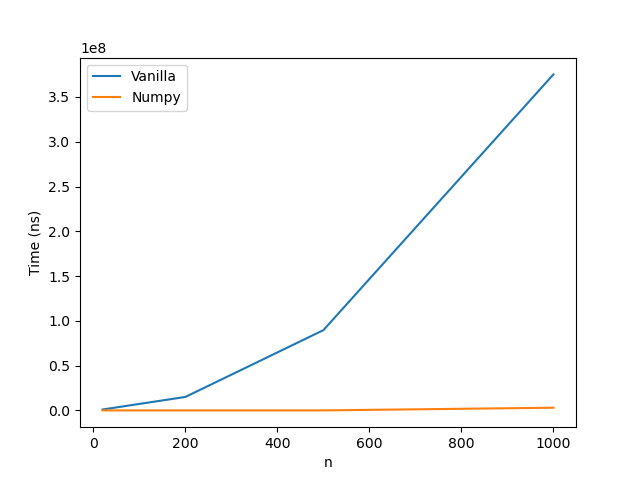
\includegraphics[scale=0.5]{wallclocktimes.png}
		\end{figure}
	
		We can see that the numpy implementation stays nearly constant while the vanilla implementation scales linearly. We know that python arrays (even of ints) are arrays of pointers that point to ints in memory, while numpy arrays are blocks in memory (like in c) and that numpy operations can take advantage of parallelism. Since my CPU has many threads, this means that the efficient usage of more threads will cut the time down drastically, while the naive python implementation will only be able to make use of a single thread.
		
		\item \begin{enumerate}
			\item The value the code gave me was $n = 40,000$. As seen in the below plot, the theoretical results of the law of large number hold up quite drastically. The empirical values of the CDF very, very quickly go to the normal distribution (even with a relatively small number of variables of $n=512$). 
			
			\item Here is my plot:
			\begin{figure}[H]
				\centering
				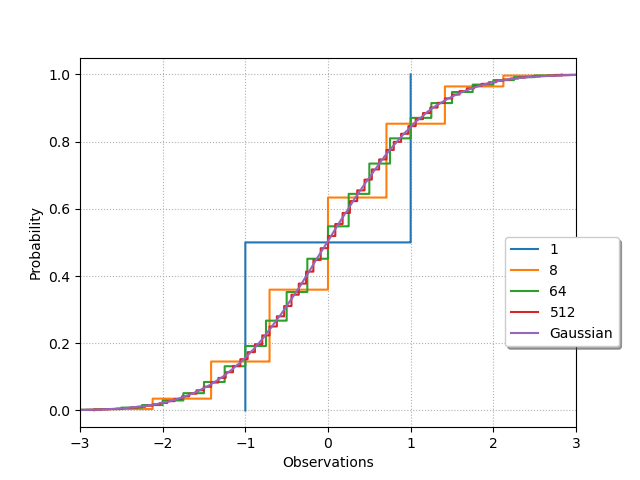
\includegraphics[scale=0.5]{gaussianplot.png}
			\end{figure}
		\end{enumerate}	
	\end{enumerate}
\end{document}